\section{Middleware}

In questa sezione viene definita la struttura degli attori presenti nel middleware, la modalità di associazione con l'entità esterna (mente e corpo) ed il collegamento interno tra attori.

\subsection{Attori}

Come illustrato nella sezione \ref{struttura_middleware} la presenza di Akka all'interno del framework Play ha portato all'utilizzo degli attori come rappresentazione di una parte dell'entità (mente/corpo) all'interno del middleware. 

\medskip

In Synapsis è definito un attore \textit{"BaseActor"} come attore generico in grado di ricevere messaggio dall'esterno, comunicare con la controparte, sempre attore, e di inviare messaggi alla propria parte di entità collegata.

\begin{figure}[H]
\centering
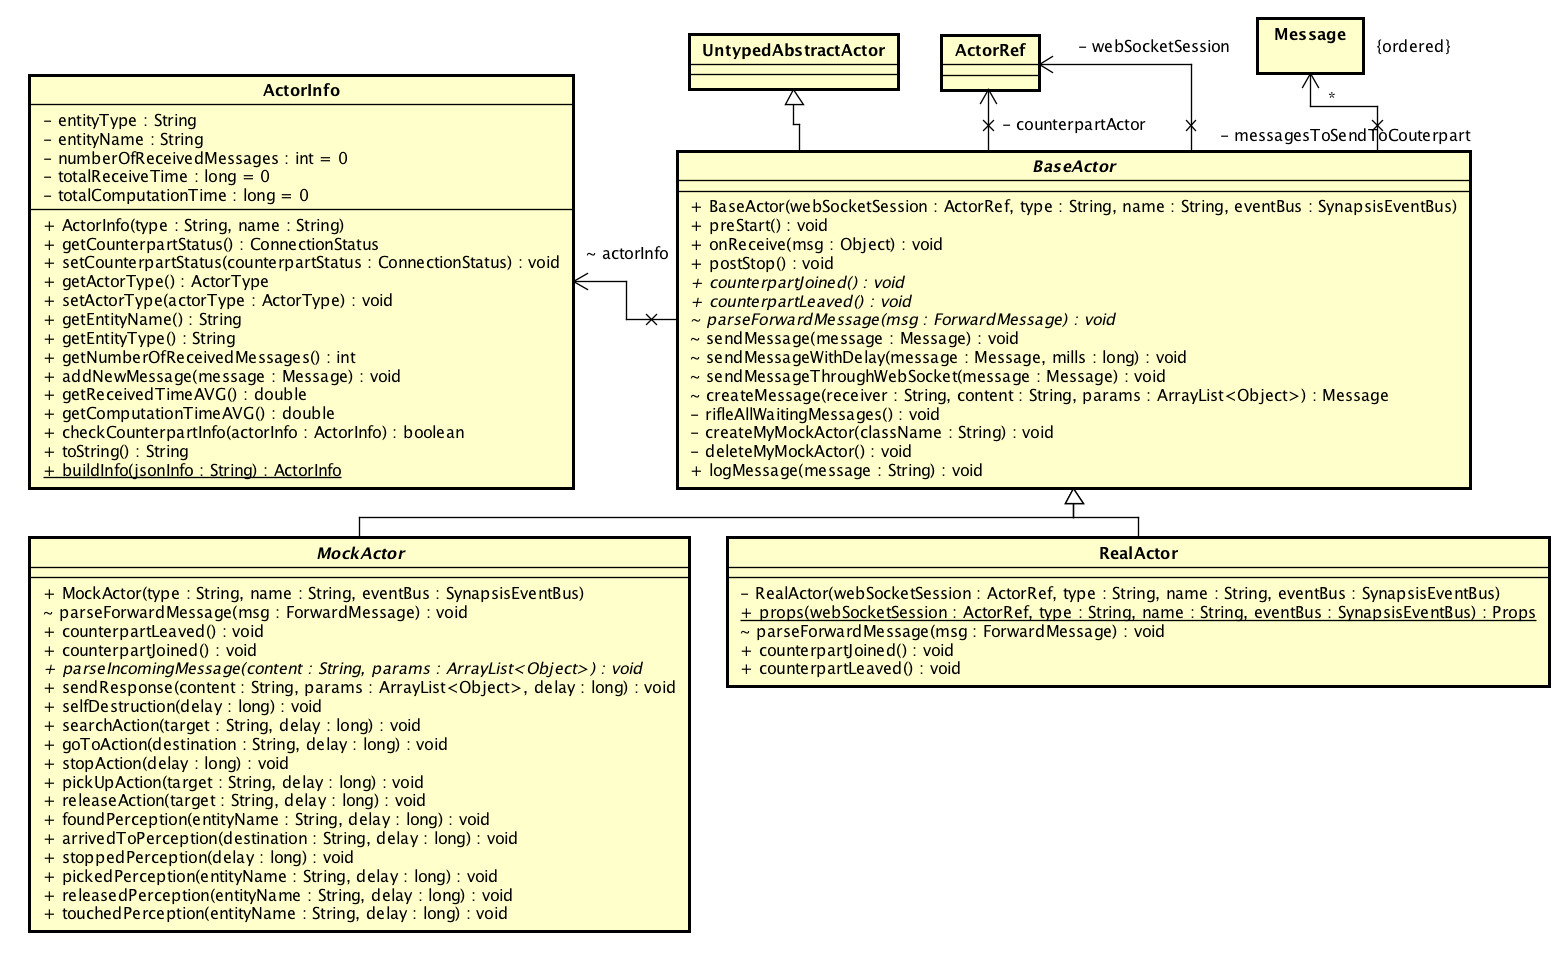
\includegraphics[width=\textwidth]{figures/diagramma_classi_attori.png}
\caption{Diagramma della classi degli attori presenti in Synapsis}
\label{classi_attori}
\end{figure}

Nella figura \ref{classi_attori} è presente il diagramma delle classi focalizzato sulla struttura degli attori all'interno di Synapsis:
\begin{itemize}
    \item \textbf{BaseActor}: classe che estende \textit{UntypedAbstractActor} e contiene i riferimenti all'attore controparte, all'entità collegata e alle funzionalità base necessarie ad un attore per svolgere il proprio compito;
    \item \textbf{ActorInfo}: classe che contiene le informazioni necessarie ad identificare un attore come nome e tipologia (mente o corpo);
    \item \textbf{RealActor}: classe che estende \textit{BaseActor} e che viene istanziata quando un'entità esterna si collega al middleware;
    \item \textbf{MockActor}: classe che estende \textit{BaseActor} utile per il rapid prototyping dato che permette di simulare un attore, e quindi una parte dell'entità senza che quest'ultima sia realmente collegata al middleware. Per approfondimenti consultare l'appendice \ref{mock_actor}.
\end{itemize}

\subsection{Collegamento tra attore e entità}

Il framework Play offre diverse modalità per rendere raggiungibile l'applicazione dall'esterno come, ad esempio, richieste HTTP sincrone, asincrone e WebSocket (WS). Queste ultime sono risultate le più adatte per effettuare il collegamento tra attore ed entità, data la possibilità di instaurare una connessione duratura e bidirezionale.

\medskip

Stabilendo un collegamento WS, Play si occupa di inglobare il canale in un attore, rendendo possibile il suo utilizzo all'interno del sistema ad attori e mettendo a disposizione dello sviluppatore il riferimento all'attore appena creato. 

\medskip

In Synapsis, questo riferimento viene passato all'effettivo attore che si occuperà di gestire i messaggi inviati dall'entità. Lo stesso procedimento viene eseguito per ogni connessione aperta, quindi, il rapporto tra numero di connessioni WS e attori "mente/corpo" è sempre di 1:1. In caso di chiusura del canale WS, Play rimuove automaticamente l'attore creato in precedenza dal sistema.

\begin{figure}[H]
\centering
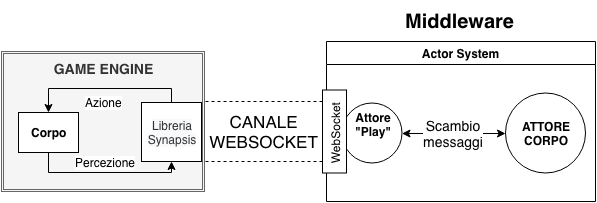
\includegraphics[width=\textwidth]{figures/Middleware_entita_attore.png}
\caption{Esempio di collegamento tra attore e entità "corpo"}
\end{figure}

\subsection{Indirizzo di collegamento al middleware}

L'utilizzo di WebSocket, come protocollo di comunicazione tra i componenti del sistema, ha necessariamente portato a definire quale tra questi svolgerà la funzione di WebSocket Server. Il framework Play supportando nativamente questo protocollo è anche configurabile come server.

\medskip

Lo standard RFC6455 stabilisce la struttura del URI che il WebSocket client utilizzerà per collegarsi alla risorsa/servizio messo a disposizione dal server. Per Synapsis è stato definito questo URI:
\begin{itemize}
    \item ws://localhost:9000/\textbf{synapsiservice}/\textit{type}/\textit{name}
\end{itemize}

L'indirizzo specifica l'utilizzo di una connessione non criptata \textit{"ws"} verso l'istanza locale dell'applicativo Play \textit{"localhost:9000"} e l'utilizzo del servizio \textit{"synapsiservice"} con l'aggiunta di parametri utili ad identificare l'entità che si collegherà a Synapsis. 

\medskip

In Play è presente un router HTTP, componente configurabile con il compito di tradurre ogni richiesta HTTP in un'azione dell'applicativo, dove configurare le rotte che l'applicazione rende utilizzabili dai client. Per il pattern MVC ogni richiesta HTTP viene tramutata in evento che invoca un determinato metodo. Ogni rotta è formata dalle seguenti componenti:
\begin{itemize}
    \item Il metodo HTTP (e.g. GET, POST, …).
    \item l'indirizzo della richiesta (e.g. /clienti/1542, /foto/lista), incluse eventuali Query
\end{itemize}

\lstinputlisting[label={playroutes},caption={File \textit{routes}, configurazione rotte su Play},]{code/routes}

Il listato \ref{playroutes} mostra il file utilizzato per definire la struttura dell'indirizzo per collegarsi al middleware e come vengono utilizzati i parametri passati in fase di instaurazione del collegamento WebSocket. Ogni entità corpo o mente per creare il collegamento WebSocket deve specificare la propria tipologia e il nome che la identifica, ad esempio se la mente dell'entità "robot" vuole collegarsi al middleware l'indirizzo che utilizzerà è il seguente:

\begin{itemize}
    \item ws://localhost:9000/synapsiservice/\textbf{mind}/\textbf{robot}
\end{itemize}

Il passaggio di questi parametri viene utilizzato dal middleware per istanziare l'attore, che rappresenta la parte di entità all'interno del sistema ad attori.

\subsection{Collegamento tra attori "mente" e "corpo"}

All'intero del sistema ad attori non è possibile inviare messaggi senza avere il riferimento al destinatario. Questo aspetto ha rappresentato un problema per il collegamento interno tra attore "mente" e attore "corpo", dato che entrambi vengono creati nel sistema ad attori successivamente all'instaurazione di un canale WS. Infatti, non è sicuro che l'entità "corpo" e l'entità "mente" si colleghino simultaneamente a Synapsis.

\medskip

L'interfaccia EventBus\footnote{presente nella libreria \href{https://doc.akka.io/docs/akka/current/event-bus.html}{Akka}}, a disposizione degli sviluppatori, permette di creare un sistema di notifiche broadcast identificate da uno specifico argomento (topic), a tutti gli attori registrati allo stesso tipo di argomento. All'interno del middleware è stata realizzata la classe \textit{SynapsisEventBus}, implementando l'interfaccia EventBus, che viene utilizzata per gestire il primo collegamento e la disconnessione tra attori della stessa entità.

\begin{figure}[H]
\centering
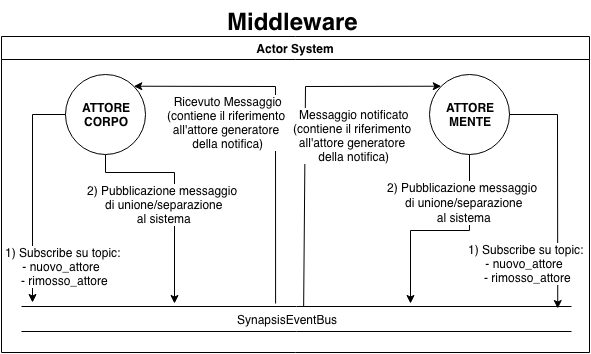
\includegraphics[width=\textwidth]{figures/SynapsisEventBus.png}
\caption{SynapsisEventBus - collegamento e disconnessione attori}
\end{figure}

Di seguito viene illustrato un esempio di funzionamento in caso di creazione dell'attore "corpo", ipotizzando che l'attore "mente" sia già presente nel sistema:
\begin{enumerate}
    \item Il nuovo attore "corpo" si sottoscrive sul SynapsisEventBus sugli argomenti \textit{"nuovo\_attore"} e \textit{"rimosso\_attore"},
    \item L'attore "corpo" pubblica su SynapsisEventBus un messaggio con argomento \textit{"nuovo\_attore"},
    \item SynapsisEventBus notifica tutti i sottoscritti a quel determinato evento con un messaggio che conterrà anche il riferimento dell'attore che ha pubblicato il messaggio,
    \item L'attore "mente" riceve il messaggio con il riferimento all'attore "corpo" e notifica nuovamente (aveva già comunicato all'EventBus la propria presenza), così da far ricevere il proprio riferimento all'attore "corpo" appena unito al sistema.
\end{enumerate}
